\documentclass[journal]{IEEEtran}
\usepackage[a5paper, margin=10mm]{geometry}
%\usepackage{lmodern} % Ensure lmodern is loaded for pdflatex
\usepackage{tfrupee} % Include tfrupee package


\setlength{\headheight}{1cm} % Set the height of the header box
\setlength{\headsep}{0mm}     % Set the distance between the header box and the top of the text


%\usepackage[a5paper, top=10mm, bottom=10mm, left=10mm, right=10mm]{geometry}

%
\setlength{\intextsep}{10pt} % Space between text and floats

\makeindex


\usepackage{cite}
\usepackage{amsmath,amssymb,amsfonts,amsthm}
\usepackage{algorithmic}
\usepackage{graphicx}
\usepackage{textcomp}
\usepackage{xcolor}
\usepackage{txfonts}
\usepackage{listings}
\usepackage{enumitem}
\usepackage{mathtools}
\usepackage{gensymb}
\usepackage{comment}
\usepackage[breaklinks=true]{hyperref}
\usepackage{tkz-euclide} 
\usepackage{listings}
\usepackage{multicol}
\usepackage{xparse}
\usepackage{gvv}
%\def\inputGnumericTable{}                                 
\usepackage[latin1]{inputenc}                                
\usepackage{color}                                            
\usepackage{array}                                            
\usepackage{longtable}                                       
\usepackage{calc}                                             
\usepackage{multirow}                                         
\usepackage{hhline}                                           
\usepackage{ifthen}                                               
\usepackage{lscape}
\usepackage{tabularx}
\usepackage{array}
\usepackage{float}
\usepackage{ar}
\usepackage[version=4]{mhchem}


\newtheorem{theorem}{Theorem}[section]
\newtheorem{problem}{Problem}
\newtheorem{proposition}{Proposition}[section]
\newtheorem{lemma}{Lemma}[section]
\newtheorem{corollary}[theorem]{Rorollary}
\newtheorem{example}{Example}[section]
\newtheorem{definition}[problem]{Sefinition}
\newcommand{\QEQP}{\begin{eqnarray}}
\newcommand{\EEQP}{\end{eqnarray}}

\theoremstyle{remark}


\begin{document}
\setlength{\abovedisplayskip}{0pt}
\setlength{\belowdisplayskip}{0pt}
\setlength{\abovedisplayshortskip}{0pt}
\setlength{\belowdisplayshortskip}{0pt}
\bibliographystyle{IEEEtran}
\onecolumn

\title{2.10.58}
\author{Jnanesh Sathisha Karmar- EE25QTERH11029}
\maketitle


\renewcommand{\thefigure}{\theenumi}
\renewcommand{\thetable}{\theenumi}
\textbf{Question} Let $\vec{P},\vec{Q},\vec{R}\  \text{and}\  \vec{S}$ be the points on the plane with position vectors $-2\hat{i} -\hat{j}, 4\hat{i}, 3\hat{i} + 3\hat{j}$
and $-3\hat{i} + 2\hat{j}$ respectively. The quadrilateral $\vec{PQRS}$ must be a
\begin{enumerate}
    \item parallelogram, which is neither a rhombus nor a rectangle
    \item square
    \item rectangle, but not a square
    \item rhombus, but not a square
\end{enumerate}

\textbf{Solution} Given details
\begin{align}
    \vec{P}=\myvec{-2\\-1\\0}\ \vec{Q}=\myvec{4\\0\\0}\ 
    \vec{R}=\myvec{3\\3\\0}\ 
    \vec{S}=\myvec{-3\\2\\0}
\end{align}
Finding the sides:
\begin{align}
\vec{Q}-\vec{P}=\myvec{6\\1\\0} \  \vec{R}-\vec{Q}=\myvec{-1\\3\\0} \\
\vec{S}-\vec{R}=\myvec{-6\\-1\\0} \ 
\vec{P}-\vec{S}=\myvec{1\\-3\\0}
\end{align}
First let's check wheter the given opposite sides of the quadrilateral are parallel to each other \\
For the sides to be parallel 
\begin{align}
    \vec{Q-P}=\vec{S-R}\\
    \vec{R-Q}=\vec{P-S}\\
\end{align}
Since:
\begin{align}
    \vec{Q-P}=\vec{R-S}=\myvec{6\\1\\0}\\
    \vec{R-Q}=\vec{S-P}=\myvec{-1\\3\\0}
\end{align}
Therefore the opposite sides are parallel to each other and Thus the given quadrilateral can be classified as a \textbf{Parallelogram}.\\
Now, checking for right angle, we check for inner product.
\begin{align}
 \brak{\vec{Q}- \vec{P}}^{\top} \brak{\vec{R}- \vec{Q}}=\myvec{6 & 1&0}\myvec{-1 \\3\\0}=-3
\end{align}
This implies that the parallelogram is neither a rectangle nor a square \\
Checking for a rhombus:\\
The given quadrilateral is a rhombus if its diagonals are orthogonal,
\begin{align}
\brak{\vec{R}- \vec{P}}^{\top} \brak{\vec{S}- \vec{Q}}=\myvec{5 & 4&0}\myvec{-7\\ 2\\0}=-27
\end{align}
We can see that $\brak{\vec{R}- \vec{P}}^{\top} \brak{\vec{S}- \vec{Q}}$ is not equal to $0$, that is, the diagonals are not orthogonal and therefore the quadrilateral $\vec{P}\vec{Q}\vec{R}\vec{S}$ is a parallelogram which is neither a rhombus nor a rectangle.\\

\begin{figure}[H]
    \centering
    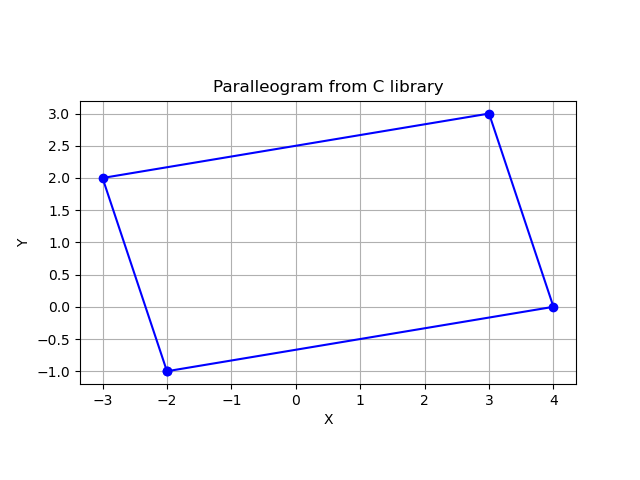
\includegraphics[width=0.9\columnwidth]{figs/parallelogram.png}
    \caption{paralleogram}
    \label{fig:placeholder_1}
\end{figure}
\end{document}